\chapter{Related Works}
\label{c:related-work}

In the following, BioCloud is compared with currently available and popular
frameworks, tools and platforms for either NGS analysis pipeline execution or
result report generation. Overall, commercial products such as DNAnexus and
Partek Flow provide more comprehensive functionalities and support than open
source projects and tools. Comparison between a larger sets of related works
can be found in \citeauthor{leipzig2016:review}'s study
\cite{leipzig2016:review}.


\section{Commercial online analysis platforms}

DNAnexus \cite{:dnanexus} is an commercial cloud-based sequencing data analysis
platform, which is undoubtedly the most feature-rich platform currently
available. The role DNAnexus plays in a typical sequencing-driven study is
illustrated in Figure~\ref{fig:dnanexus-workflow}. It covers sequencing samples
management, online analysis pipeline execution, and a result view integrated
with its custom crafted genome browser. All of its functionalities are designed
to be user friendly and does require little understanding of programming and
how to mangle with multiple sequencing formats. However, due to its by-design
simplicity, user can not easily customize their own pipeline to adopt new
published tools or update the tool version in use. On top of that, the usage of
clinical data may be subjected to different law restrictions in different
countries. Using service and cloud sever hosted and managed by a United States
company may not meet the law restrictions in Taiwan and raises extra concern
and private issues for hosting data with patient and clinical information.

\begin{figure}[!htbp]
\centering
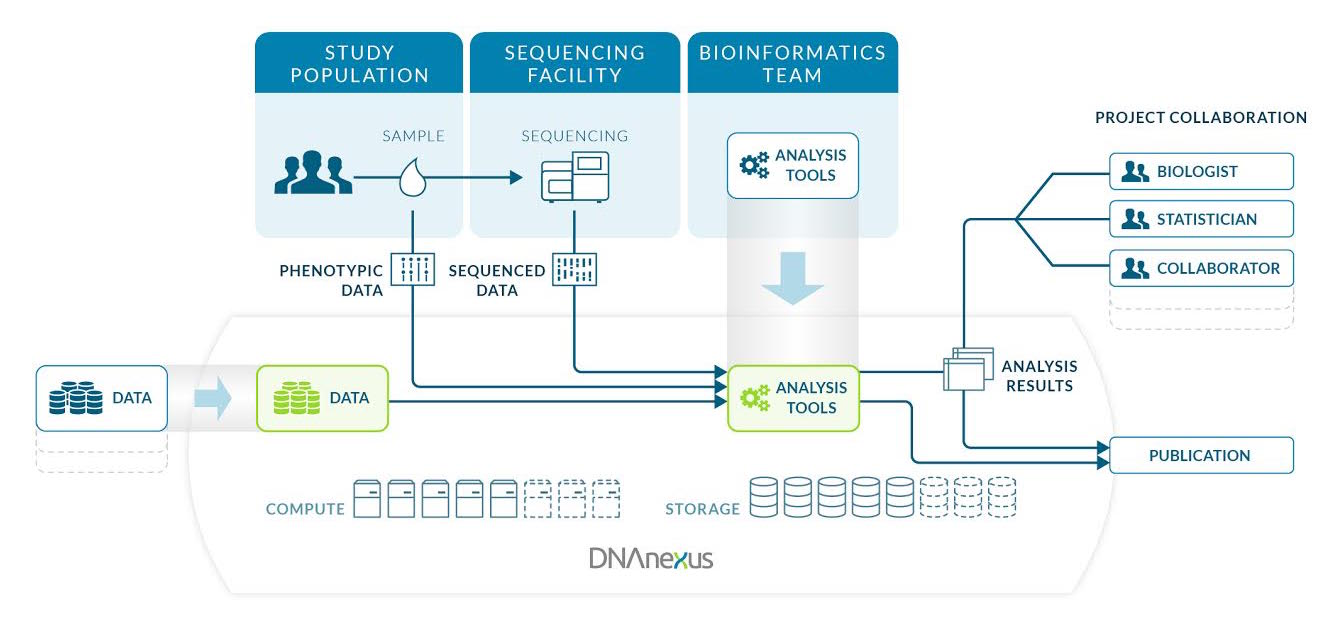
\includegraphics[width=\textwidth]{images/dnanexus_workflow}
\caption[DNAnexus workflow]{
    The role of DNAnexus in a typical sequencing-driven study. User or the
    sequencing facility can upload raw sequencing samples to the DNAnexus and
    complete the rest of the analysis on its platform. The workflow is obtained
    from \href
    {https://www.dnanexus.com/images/diagram/img-platform-genome.jpg}
    {DNAnexus's official website}.
}
\label{fig:dnanexus-workflow}
\end{figure}


Another commercial product, Partek Flow \cite{:partek}, focus more oriented to
bioinformatic researchers by offering custom pipeline design and online
analysis pipeline execution. An example of the custom pipeline design on Partek
Flow is shown in Figure~\ref{fig:partek-flow-pipeline}. User can drag and drop
different function blocks from its tool panel and connect them as a pipeline,
which is very flexible for researchers to explore different combinations of
tools. For different function blocks they can append with different type of
reports or quality assessment. The whole system can be hosted on one's own
server. Due to its flexibility of pipeline design, however, Partek Flow user
should be familiar with all analysis tools involved before conducting new
analysis. Though viewed convenient by bioinformatic researchers, it has a
relatively complex interface to design and execute analysis pipelines.

% TODO: update with our lab's screenshot
\begin{figure}[!htbp]
\centering
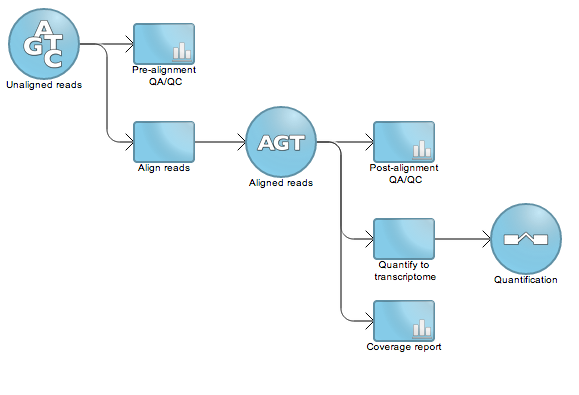
\includegraphics[width=0.7\textwidth]{images/partek_flow_pipeline}
\caption[Example of custom pipeline design on Partek Flow]{
    Example of custom RNA-Seq analysis pipeline design on Partek Flow. It first
    use gnome aligner STAR to align the sequencing, and then use Cufflinks
    quantify the transcript expression. Pre-alignment and post-alignment
    quality check are added. An alignment coverage report is added after
    alignment. The custom pipeline is obtained from
    \href{http://www.partek.com/star-align-and-quantify}{Partek Flow's official site}.
}
\label{fig:partek-flow-pipeline}
\end{figure}




\section{Open sourced online analysis platform}

The Galaxy project \cite{goecks2010:galaxy} is the most widely used general
purpose bioinformatic analysis platform, which aims for reproducible research
in computational biology. Like commercial platforms previously mentioned,
Galaxy can let user upload and manage their own data sources, execute tools
remotely, and convert the execution history into reproducible workflow via its
flexible workflow editor. Galaxy can be deployed on one's own cloud or server,
while they also maintain a list of public Galaxy servers with commonly used
toolboxes to let anyone to try on freely. Support for NGS data analysis has
reached a relatively mature state where most common tools are available and can
be accessed on their public servers. Figure~\ref{fig:galaxy-workflow} shows how
a typical RNA-Seq analysis workflow called Tuxedo looks like in Galaxy's
workflow editor, which best demonstrates the powerfulness and flexibility the
editor provides. However, it is more specifically designed for bioinformatic
researchers than Partek Flow. Also it has been developed for years, some of the
Galaxy dependencies make its source code obscure for normal Python developers,
which they often craft their own tool chains without adopting language agnostic
standards. A pile of specially developed tool chains make the Galaxy plugin
development more difficult then it seems at first. It may also lead to security
issues since most of their own developed web tools have not been publicly
battle tested, whereas standard Python web frameworks and tools like Flask and
Django have been audited and publicly tested by worldwide companies for years.

\begin{figure}[!htbp]
\centering
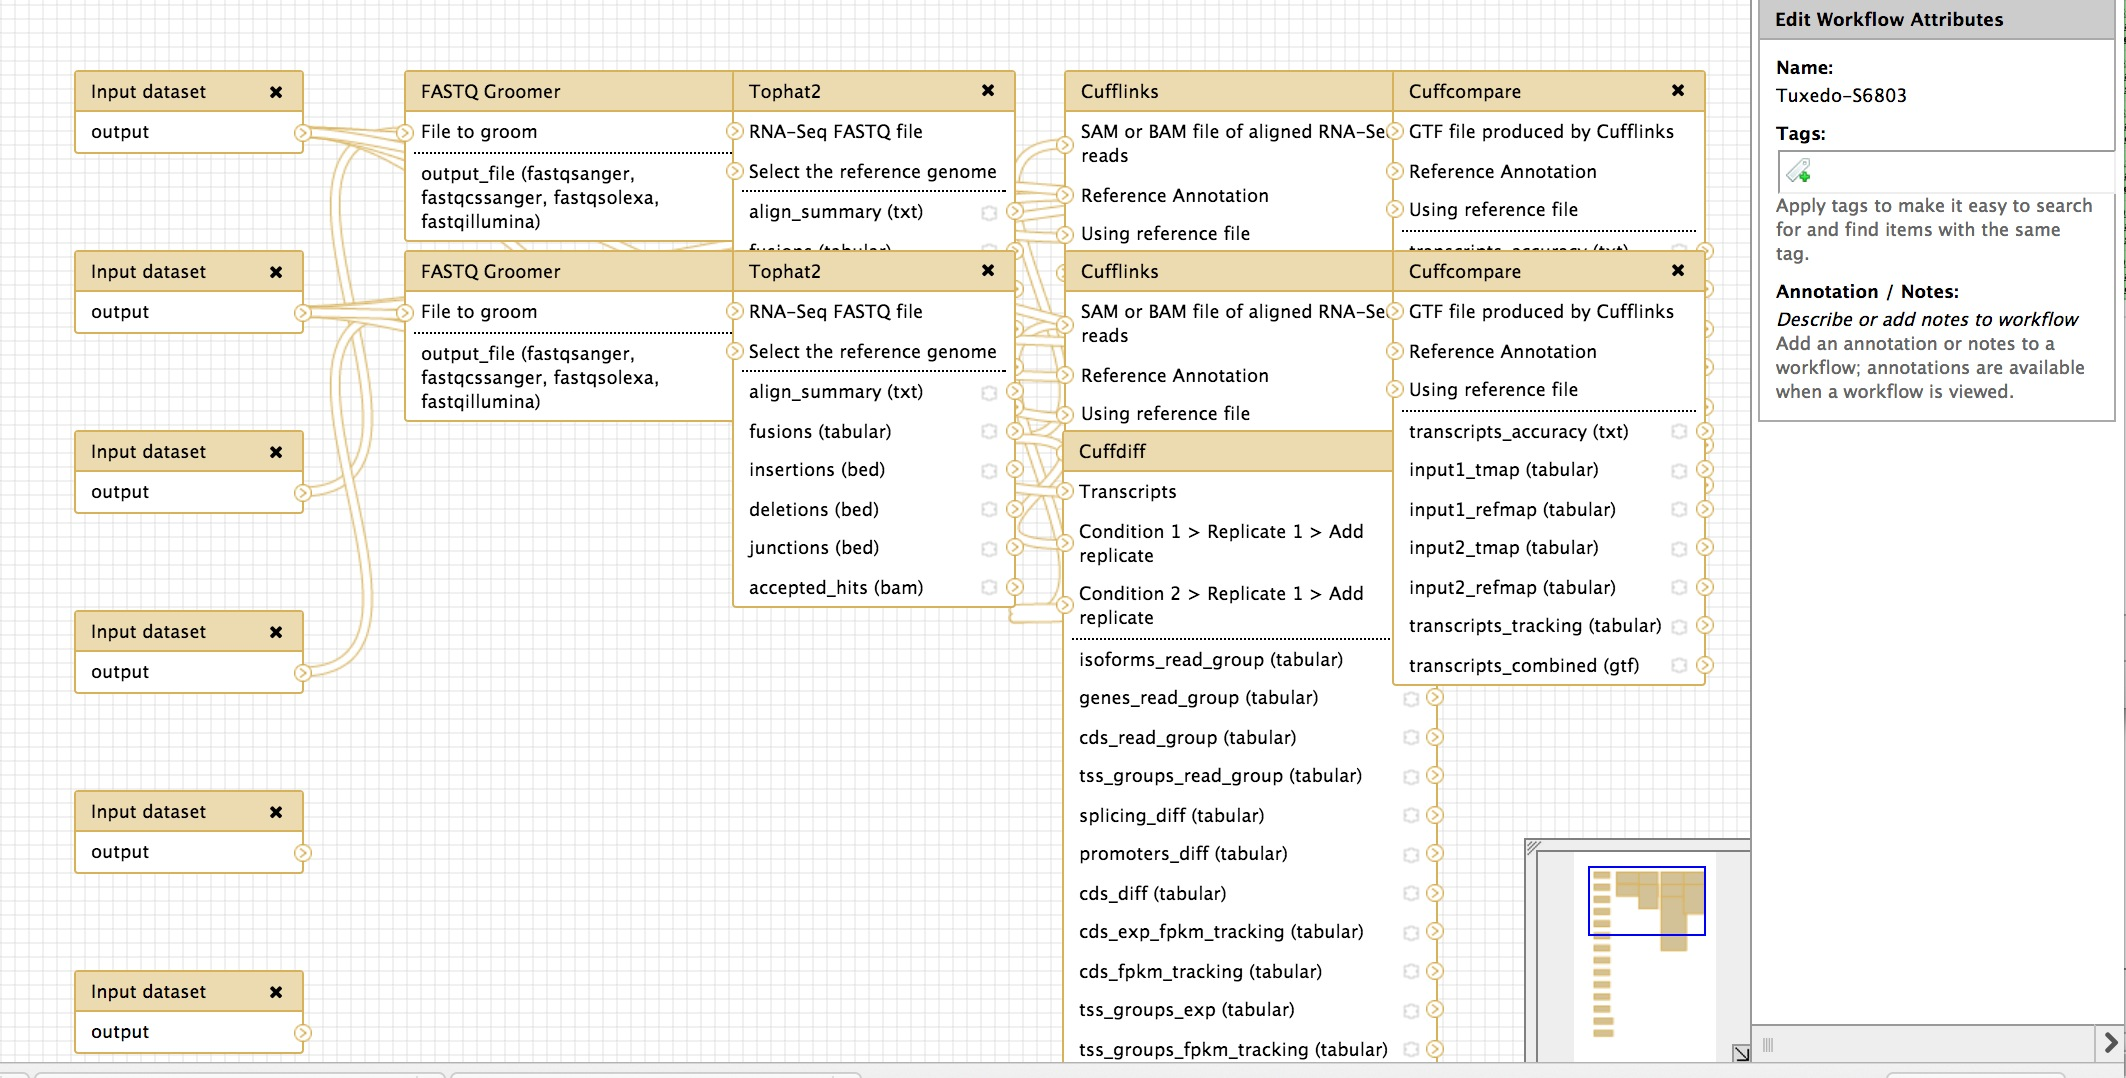
\includegraphics[width=1\textwidth]{images/galaxy_workflow}
\caption[Example of custom workflow on Galaxy]{
    Example of custom workflow on Galaxy implementing the Tuxedo RNA-Seq
    analysis workflow. This RNA-Seq workflow uses Tophat2 as genome aligner and
    Cufflinks for transcript expression inference. The shown custom workflow is
    developed and obtained from
        \href{http://genomeintelligence.org/?p=561}
        {Genome Intelligene website}
    made by Dr. Cynthia Gibas.
}
\label{fig:galaxy-workflow}
\end{figure}




Another sequencing analysis platform, Genome Modeling System
\cite{griffith2015:genome}, is used in The Genome Institute of Washington
University and has process hundreds of terabytes of sequencing data with
predefined hundreds of bioinformatic tool profiles. It resembles Galaxy in the
flexibility of developing custom workflow, while focusing solely on processing
sequencing data. Using the terminology of Genome Modeling System, sequencing
sources are subjects, and user can define multiple genome model on the same set
of subject. Genome model is defined by connections of tool profiles. Tool of
different versions have different profiles to ensure the result of genome model
can be strictly reproducible using pinned version of tools. However, like
Galaxy, it has a relatively complex design of pipeline design and does not suit
for biological researchers and clinicians.


\section{Pipeline execution tools}

Though some of the works are not a full-fledged online analysis platform, they
focus on the automated analysis pipeline design, including bcbio-nextgen
\cite{:bcbionextgen,guimera2012:bcbionextgen} and Snakemake
\cite{koster2012:snakemakea}, whose architecture designs either share common
traits with BioCloud or inspire some features of BioCloud.

In bcbio-nextgen \cite{:bcbionextgen,guimera2012:bcbionextgen}, user can adopt
existed or design custom analysis type, and then specify the input samples,
genome reference, and other necessary parameters through a pipeline
configuration file in YAML format, which is human readable and simple to write
from scratch in plain text. An configuration example of RNA-Seq analysis is
shown in Listing~\ref{lst:bcbio-nextgen-config}, whose structure and syntax
share plenty of common with BioCloud's analysis configuration file.
Bcbio-nextgen by default ships with predefined of DNA-Seq, RNA-Seq, small
RNA-Seq, and CHIP-Seq pipelines so real analysis can be performed with little
effort. The pipeline execution can utilize multi-core processors and even scale
across multiple machines through IPython Parallel framework
\cite{:ipython-parallel}. Scripts to deploy on Amazon Web Service (AWS) are
available so user can scale up the number of AWS computing instances
dynamically when needed. Bcbio-nextgen is also gradually adding support of
Common Workflow Language \cite{amstutz2016:common}, which is a on-going
workflow specification standard proposed by multiple analysis platform vendors.
The integration of IPython Parallel framework and AWS cloud infrastructure
makes bcbio-nextgen a competitive tools to perform large scale and parallel
pipeline analysis.

\begin{lstlisting}[
    caption={
        Example of bcbio-nextgen pipeline configuration to run Tophat2 genome
        alignment. The configuration is obtained from the
        \href{https://bcbio-nextgen.readthedocs.io/}
        {official tutorial of bcbio-nextgen}.
    },
    label={lst:bcbio-nextgen-config},
    language={},
]
fc_date: '070113'
fc_name: control_experiment
upload:
    dir: final
details:
    - files: [
          /full/path/to/control_1.fastq,
          /full/path/to/control_2.fastq
      ]
      description: 'Control_rep1'
      genome_build: GRCh37
      analysis: RNA-seq
      algorithm:
           aligner: tophat2
           quality_format: Standard
           trim_reads: read_through
           adapters: [truseq, polya]
           strandedness: unstranded
\end{lstlisting}

Snakemake \cite{koster2012:snakemakea} is a low-level pipeline execution tool
which is inspired by source code build automation tool Make \cite{:gnu-make}
and its rule file format Makefile. User constructs a Snakemake pipeline by
writing a series of rules which each rule corresponds to commands of a tool.
Each rule also defines its input and output file patterns, which Snakemake will
use them to construct the execution dependencies between rules as a directed
acyclic graph (DAG). Listing~\ref{lst:snakemake-rule} shows an example of
writing Snakemake rule to run BWA MEM genome alignment. Like Makefile, the
variable \texttt{\{sample\}} specified in the input FASTQ files will be auto
expanded to all files matching the given pattern, that is, all files with
suffix \texttt{.fastq} under the folder \texttt{data/samples/}.  Before
execution, these rules are first evaluated and expanded to all matched files to
build the DAG dependencies, shown in Figure~\ref{fig:snakemake-dag}.  Snakemake
will detect outdated output files by comparing creation timestamp with input
files. Only outdated outputs will be re-executed, which reduces the total
execution time. Other parameters of the Snakemake rule can further control the
resources a job can use, e.g., number of threads and read-only files to prevent
output files from being rewritten.

\begin{lstlisting}[
    caption={
        Example of Snakemake rule to run BWA MEM genome alignment. The rule is
        obtained from the
        \href{http://snakemake.bitbucket.org/snakemake-tutorial.html}
            {official tutorial of Snakemake}.
    },
    label={lst:snakemake-rule},
    language={},
]
rule bwa_map:
    input:
        "data/genome.fa",
        "data/samples/{sample}.fastq"
    output:
        "mapped_reads/{sample}.bam"
    shell:
        "bwa mem {input} | samtools view -Sb - > {output}"
\end{lstlisting}

\begin{figure}[!htbp]
\centering
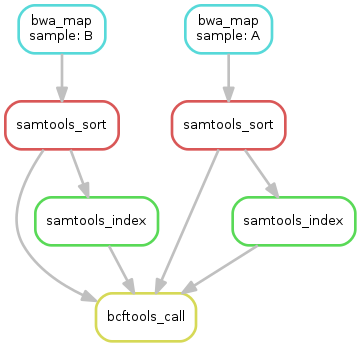
\includegraphics[width=0.5\textwidth]{images/snakemake_dag}
\caption[Example of DAG job dependencies of a Snakemake workflow]{
    Example of DAG job dependencies of a Snakemake workflow that first aligns
    sequence reads to genome using BWA MEM, sorts and indexes the aligned BAM
    file, and finally calls variants using bcftools. Two samples A and B are
    used, and Snakemake can correctly understand the input and output
    dependencies for each job through file expansion and collection rule. The
    workflow is obtained from
    \href{http://snakemake.bitbucket.org/snakemake-tutorial.html}
    {the official tutorial of Snakemake}.
}
\label{fig:snakemake-dag}
\end{figure}




Though Snakemake may not be directly used by biological researchers and
clinicians, integrating it into a cloud platform may not be as trivial as it
seems. Monitoring the Snakemake execution process can be complicated since it
treats individual inputs as separate jobs. One could either show the detailed
execution progress or trying to deep integrate with Snakemake to collect all
the job details and organize them externally. The latter deep integration can
be easily broken if Snakemake changes its internal structure.

Two pipeline execution tools mentioned above can be used as the way Biocloud
run analysis pipelines. However, due to time constraint and development
complexity a developer can manage, BioCloud rolls out its only basic pipeline
execution method with stage monitoring. There are possibilities for BioCloud to
leverage these pipeline execution tools in future and such integrations are
discussed in Chapter \ref{c:discussion}.


\section{Analysis report generation}

An analysis report helps summarize the result of a sequencing analysis pipeline
across different samples or even different conditions in the experiment design.
Without getting into details, summary report collects the most important
statistics and results of each tools, which is suitable to provide researchers
with little sequencing experience a basic understanding the condition of one's
sequencing results.

Aside from commercial products which more or less provide a summary report,
some open sourced works also focus on the summarization of the sequencing
analysis. MultiQC \cite{ewels2016:multiqc} is a quality assessment tool for
sequencing data. After its first release in Nov 2015 it has been gaining
popularity. At the time of writing, both bcbio-nextgen and Galaxy can integrate
with MultiQC report. An example of the MultiQC report is shown in
Figure~\ref{fig:multiqc-report}, which is a single page HTML report. The first
general information table collects important statistics of each sample produced
by each tools, which user can select which of them should be displayed by
tweaking the column visibility. Following the general information, the report
shows interactive figures which user can zoom in and out, filter unwanted
samples, and export current figure state as static JPEG or PNG picture format.

However, since MultiQC focuses on quality assessment, it cannot parse the end
results of typical sequencing analysis. MultiQC treats samples independently,
so user cannot group samples of same conditions or compare samples grouped by
their conditions. For example, it cannot display the differentially expressed
genes and genomic variants called in all samples of the same condition. Also,
due to its single page web structure, showing figures of too many stages will
impact the viewing experience due to low rendering frame rate. Though MultiQC
does provide innovative ways to display sequencing results, BioCloud cannot
directly integrate MultiQC and need to develop its own way displaying figures
considering sample grouping.

\begin{figure}[p]
\centering
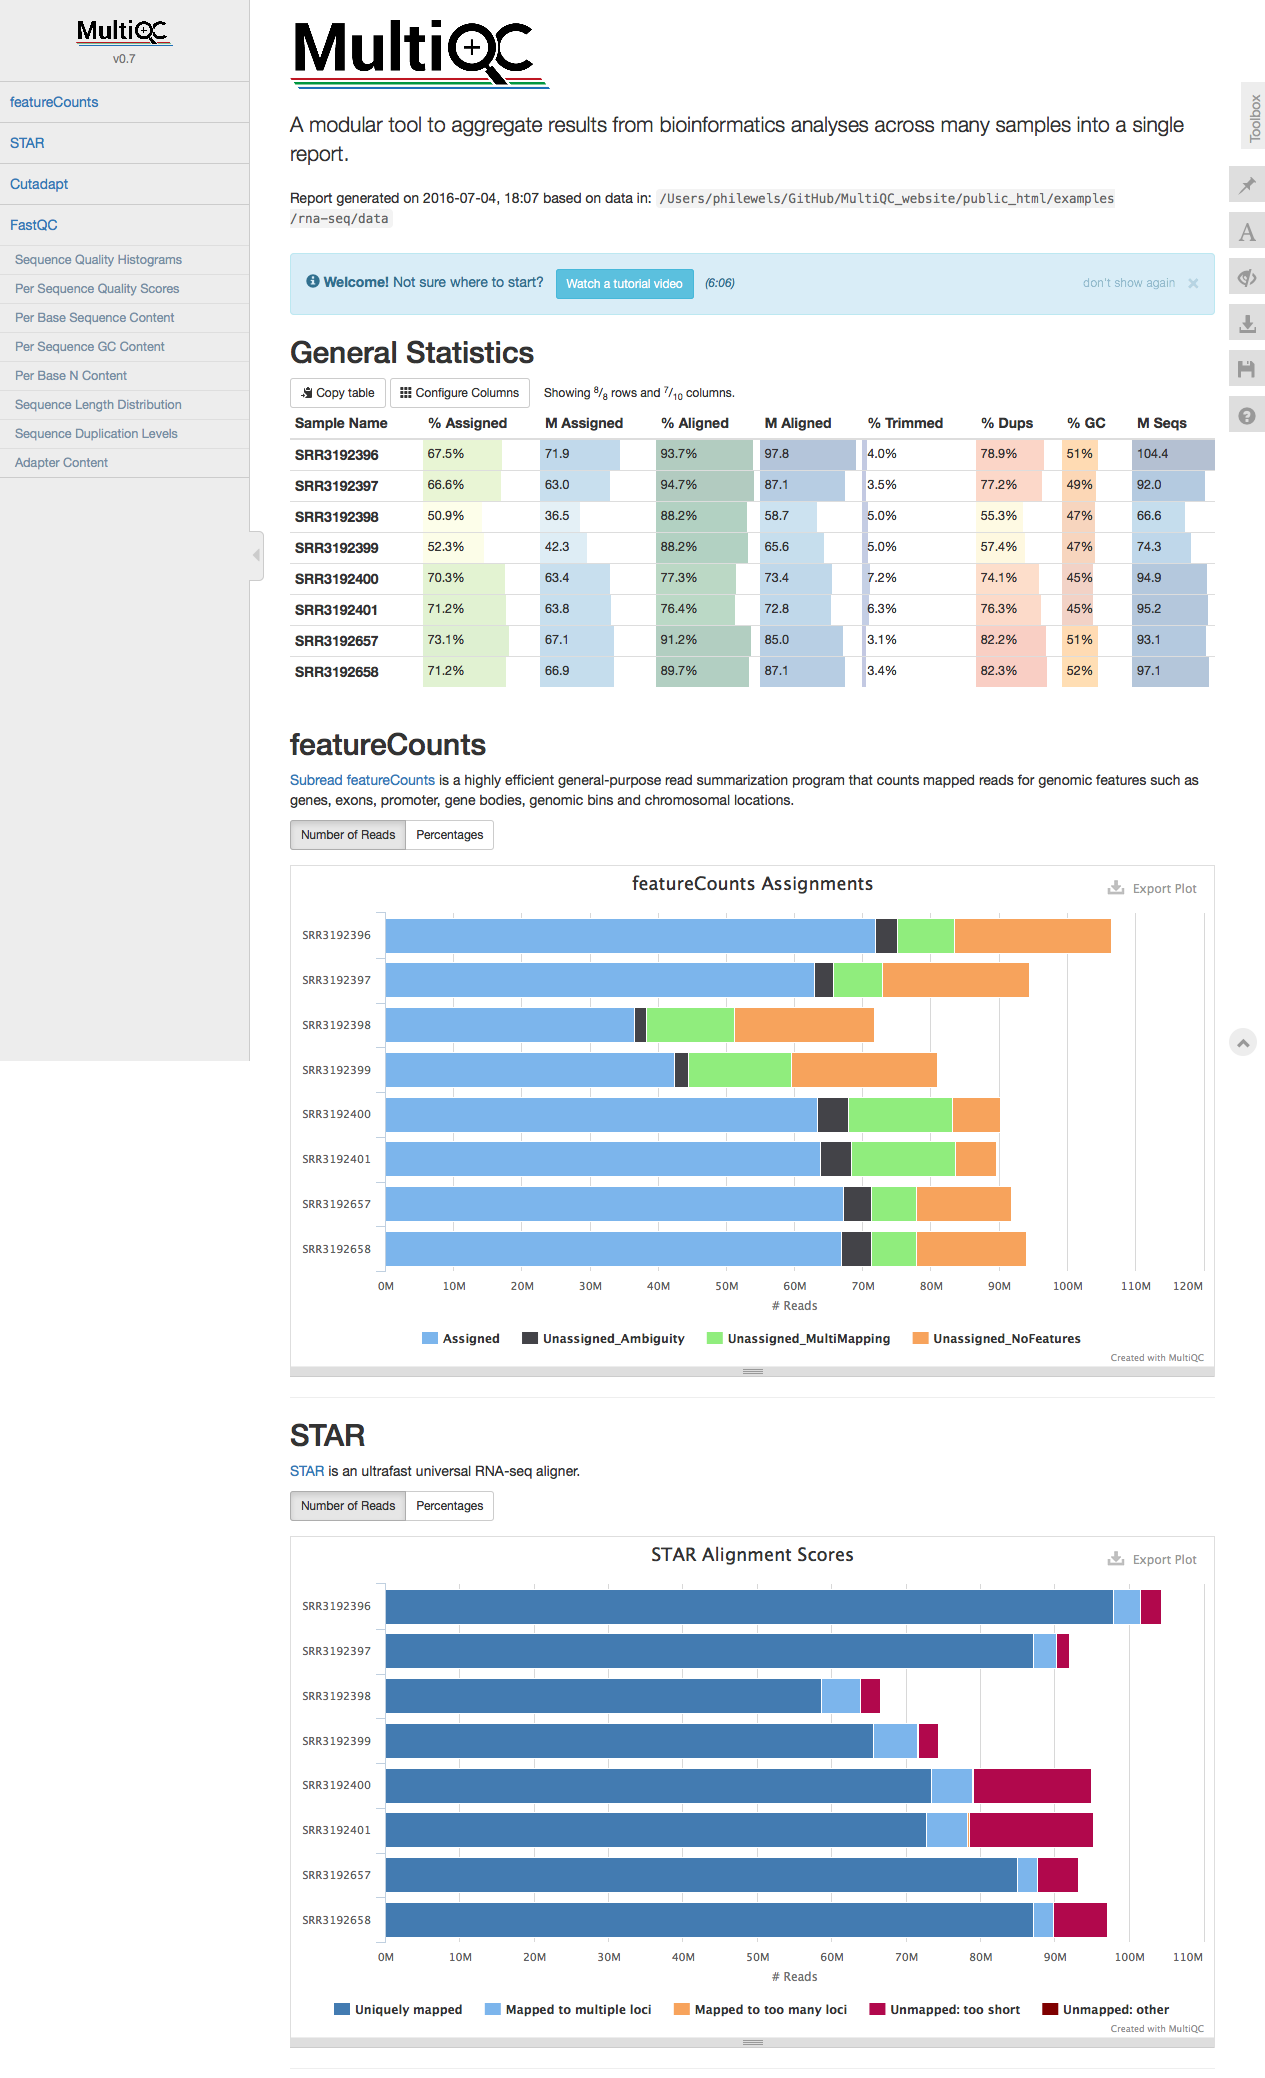
\includegraphics[width=0.9\textwidth]{images/multiqc_report}
\caption[Example MultiQC report]{
    Example MulitQC report for RNA-Seq analysis.
}
\label{fig:multiqc-report}
\end{figure}




% vim: set textwidth=79:
